% CVPR 2022 Paper Template
% based on the CVPR template provided by Ming-Ming Cheng (https://github.com/MCG-NKU/CVPR_Template)
% modified and extended by Stefan Roth (stefan.roth@NOSPAMtu-darmstadt.de)

\documentclass[10pt,twocolumn,letterpaper]{article}

%%%%%%%%% PAPER TYPE  - PLEASE UPDATE FOR FINAL VERSION
\usepackage[review]{cvpr}      % To produce the REVIEW version
%\usepackage{cvpr}              % To produce the CAMERA-READY version
%\usepackage[pagenumbers]{cvpr} % To force page numbers, e.g. for an arXiv version

% Include other packages here, before hyperref.
\usepackage{graphicx}
\usepackage{amsmath}
\usepackage{amssymb}
\usepackage{booktabs}


% It is strongly recommended to use hyperref, especially for the review version.
% hyperref with option pagebackref eases the reviewers' job.
% Please disable hyperref *only* if you encounter grave issues, e.g. with the
% file validation for the camera-ready version.
%
% If you comment hyperref and then uncomment it, you should delete
% ReviewTempalte.aux before re-running LaTeX.
% (Or just hit 'q' on the first LaTeX run, let it finish, and you
%  should be clear).
\usepackage[pagebackref,breaklinks,colorlinks]{hyperref}


% Support for easy cross-referencing
\usepackage[capitalize]{cleveref}
\crefname{section}{Sec.}{Secs.}
\Crefname{section}{Section}{Sections}
\Crefname{table}{Table}{Tables}
\crefname{table}{Tab.}{Tabs.}


%%%%%%%%% PAPER ID  - PLEASE UPDATE
\def\cvprPaperID{*****} % *** Enter the CVPR Paper ID here
\def\confName{CVPR}
\def\confYear{2022}


\begin{document}

%%%%%%%%% TITLE - PLEASE UPDATE
\title{Task-Oriented Dialog System : A Survey}

\author{First Author\\
Institution1\\
Institution1 address\\
{\tt\small firstauthor@i1.org}
% For a paper whose authors are all at the same institution,
% omit the following lines up until the closing ``}''.
% Additional authors and addresses can be added with ``\and'',
% just like the second author.
% To save space, use either the email address or home page, not both
\and
Second Author\\
Institution2\\
First line of institution2 address\\
{\tt\small secondauthor@i2.org}
}
\maketitle

%%%%%%%%% ABSTRACT
\begin{abstract}
Due to the significance and value in human-computer interaction and natural language processing, task-oriented dialog system is a hot research topic recently. In this paper, we aim to provide a survey on various task-oriented dialog system methods. Firstly, the popular methods of task-oriented dialog system are introduces in details. Secondly, we review the recent progresses in dialog evaluation. Thirdly, we discuss three dominant challenges for task-oriented dialog system. Finally, the future open research problems for task-oriented dialog system are pointed out.

\end{abstract}

%%%%%%%%% BODY TEXT
\section{Introduction}
\label{sec:intro}

Building a task-oriented dialogue system has become a hot topic in the research community and industry. The task-oriented dialogue system is designed to help users complete certain tasks in specific fields, such as restaurant reservations, weather inquiries, and flight reservations, which makes it very valuable for real-world businesses. Compared with open-domain dialogue systems whose main goal is to maximize user participation \cite{huang2020challenges}, task-oriented dialogue systems are more inclined to complete certain tasks in one or more domains. Usually, task-oriented dialogue systems are built on a structured ontology, which defines the domain knowledge of the task.

Task-oriented dialog systems are divided by architecture into two categories. One type is a pipeline system that has a modular structure, as shown in Figure \ref{pipelineframework}. It consists of four key modules:
\begin{itemize}
\item Natural Language Understanding (NLU): It identifies and parses a user’s text input to obtain semantic tags that can be understood by computers, such as slot values and intentions.
\item Dialog State Tracking (DST): It maintains the current dialog state based on the dialog history. The dialog state is the cumulative meaning of the dialog history, which is generally expressed as slot-value pairs.
\item Dialog Policy: It outputs the next system action based on the current dialog state. The DST module and the dialog policy module are collectively referred to as the dialog manager (DM).
\item Natural Language Generation (NLG): It converts system actions to natural language output.
\end{itemize}
\begin{figure*}
    \centering
    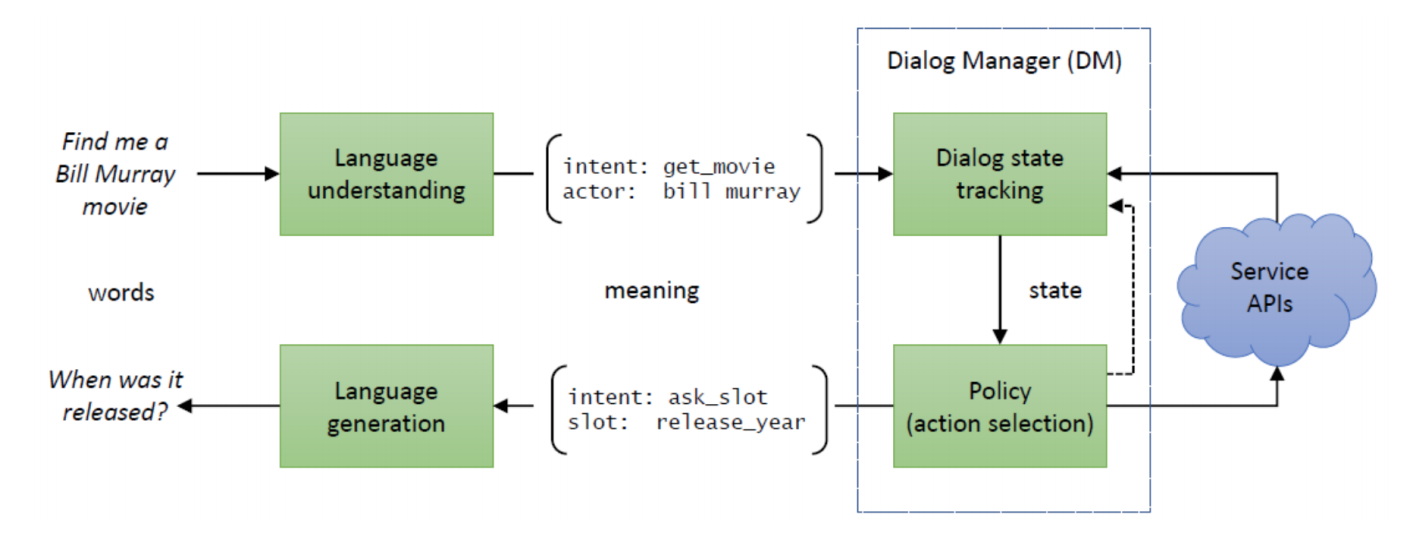
\includegraphics[scale=0.6]{pipelineframework.png}
    \caption{Modular structure of a task-oriented dialog system}
    \label{pipelineframework}
\end{figure*}
This modular system structure is highly interpretable, easy to implement, and suitable for most practical task-oriented dialogue systems in the industry. However, this structure does not flexible enough. The modules are independent of each other and it is difficult to optimize together. This makes it difficult to adapt to changing application scenarios. In addition, due to the accumulation of errors between modules, the upgrade of a single module may require adjustment of the entire system.

Another implementation of a task-oriented dialog system is an end-to-end system, which has been a popular field of academic research in recent years\cite{DBLP:conf/eacl/Rojas-BarahonaG17,madotto2018mem2seq,eric2017key,lei2018sequicity}.  This type of structure trains an overall mapping relationship from the natural language input on the user side to the natural language output on the machine side. It is highly flexible and scalable, reducing labor costs for design and removing the isolation between modules. However, the end-to-end model places high requirements on the quantity and quality of data and does not provide clear modeling for processes such as slot filling and API calling. This model is still being explored and is as yet rarely applied in the industry

This paper aims to (1) give an overview about task-oriented dialogue systems especially recent advances from deep learning; and (2) discuss possible research directions. The remaining of the article is organized as follows. 
In section 2, we review task-oriented dialogue systems including pipeline and end- to-end methods. In Section 3, we discuss recent work on task-oriented dialog evaluation, including automatic, simulated, and human evaluation methods. In Section 4, we discuss challenges in this domain and existing works proposed to solve this challenges.  In Section 5, we conclude the paper and discuss future research trends.

\section{Models and Approaches}
\subsection{Pipeline Methods}


\subsubsection{Language Understanding}
Natural language understanding(NLU) typically involves identifying a user’s intent and extracting relevant semantic constituents from the natural language sentence. It typically consists of two tasks: intent detection and slot filling\cite{tur2011spoken}. While the intent detection is a standard classification problem where one label is predicted for each sentence, slot filling is often formulated as a sequence labelling task, where a sequence of labels need to be assigned jointly.

\textbf{Intent Detection}
Given input utterance $X=(x_1, ..., x_n)$(n denotes the length of X), intent detection (ID) can be considered as a sentence classification task to decide the intent label $o^I$, which is formulated as:
\begin{equation}
    o^I = Intent-Detection(X)
    \label{eq: ID}
\end{equation}
Many sentence classification methods have been investigated for intent detection. Xu and Sarikaya\cite{xu2013convolutional} used Convolutional Neural Network to extract 5-gram features and apply max-pooling to obtain work representations, which handles intent detection and slot filling simultaneously. Ravuri and Stolcke\cite{ravuri2015recurrent} successfully applied  Recurrent Neural Network(RNN) and Long Short-Term Memory Network to intent detection task, which indicates the sequential features are beneficial to this task.

\textbf{Slot Filling}
Slot filling can be seen as a sequence labeling task to produce a sequence slots $o^S = (o_1^S,...,o_n^S)$, which can be rewritten as:
\begin{equation}
    o^S = Slot-Filling(X)
    \label{eq:SF}
\end{equation}
Popular neural approaches for slot filling includes  Conditional Random Field(CRF),  Recurrent  neural  network  (RNN)  and  RNN-based  models. 
Yao et al. \cite{yao2013recurrent} take words as input as in a standard Recurrent Neural Network Language Models(RNN-LM), and then to predict slot labels rather than words on the output side. Mesnil et al. \cite{mesnil2013investigation} carried out an in-depth investigation on the use of recurrent neural networks including Elman RNN, Jordan RNN and its bi-directional version for NLU. Yao et al. \cite{yao2014spoken} have presented an application of LSTMs to spoken language understanding for the slot filling task. Yao et al.  \cite{yao2014recurrent} have demonstrated that RNNs can be successfully merged with CRFs to do language understanding. The combination of RNN and CRF, recurrent conditional random field (R-CRF) is proved that can tackle label bias. Liu and Lane \cite{liu2015recurrent} proposed to model slot label dependencies using a sampling approach, by feeding sampled output labels (true or predicted) back to the sequence state. Vuetal \cite{vu2016bi} utilized ranking loss function on bi-RNN model in slot filling, further enhancing performance in ATIS dataset. Kurataetal \cite{kurata2016leveraging} proposed an encoder-labeler LSTM that can conduct slot filling conditioned on the encoded sentence-level information.
\begin{figure*}
    \centering
    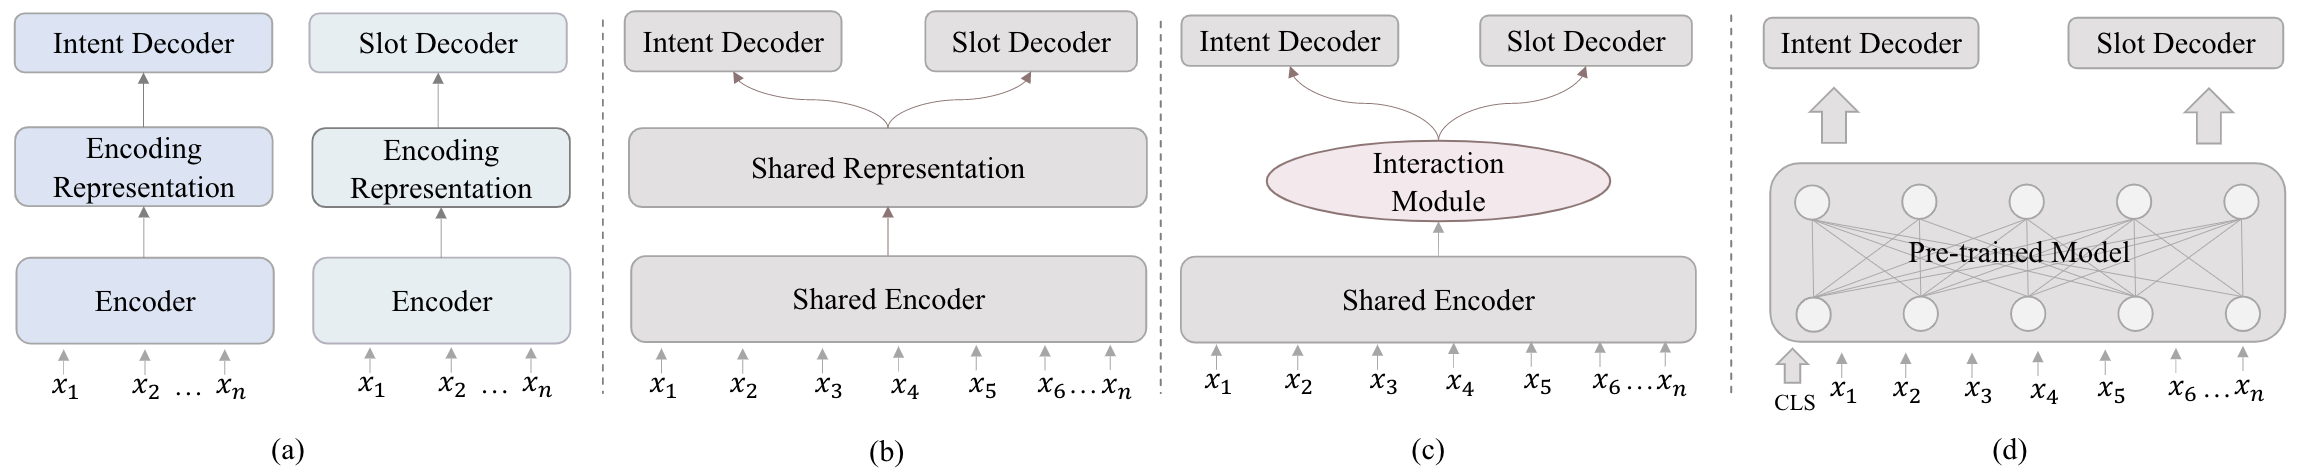
\includegraphics[scale=0.4]{NLUframework.png}
    \caption{(a) Single models. (b) Implicit Joint Modeling. (c) Explicit Joint Modeling. (d) Pre-trained Model Paradigm}
    \label{fig:NLUframework}
\end{figure*}
\textbf{Joint Models}
Considering the close correlation between intent detection and slot filling, dominant work in the literature adopts joint model to leverage the shared knowledge across tasks. Existing joint work can be classified into two main categories:implicit joint modeling and explicit joint modeling. 

Implicit joint modeling denotes that model only adopts a shared encoder to capture shared features, without any explicit interaction, which is illustrated in Figure \ref{fig:NLUframework}(b). Zhang and Wang \cite{zhang2016joint} introduced a shared RNNs (Joint ID and SF) to learn the correlation between intent and slots. Liu and Lane\cite{liu2016attention} propose an attention-based
neural network model for joint intent detection and slot filling (Attention BiRNN). Liu and Lane \cite{liu2016joint} used a shared RNN to jointly performs intent detection, slot filling, and language modeling, aiming to improve the ability of online prediction. Hakkani-Tür et al. \cite{hakkani2016multi} proposed a shared RNN-LSTM architecture (Joint Seq) forjoint modeling.

In recent years, explicitly joint modeling has attracted more and more attention. It focus on the interaction between the indent detection and slot filling with an explicit interaction module, which is shown in Figure \ref{fig:NLUframework}(c). This explicit modeling mode has the advantages of explicitly controlling process of interaction. Goo et al.\cite{goo2018slot} focuses on learning the explicit slot-intent relations by introducing a slot-gated mechanism into the state-of-the-art attention model. Qin et al.\cite{qin2019stack}  propose a joint model for spoken language understanding with Stack-Propagation to better incorporate the intent information for slot filling. Wang et al. \cite{wang2018bi} proposed  a novel Bi-model based RNN semantic frame parsing model for intent detection and slot filling. Zhang et al.\cite{zhang2018joint} introduced a novel module to harness the hierarchical relationships among words, slots, and
intents in the utterance for joint slot filling and intent detection.

Recently, Pre-trained Language Models (PLMs) achieve surprising results across various NLP tasks. Some BERT-based\cite{devlin2018bert} pre-trained work has been explored in NLU direction where a shared BERT is considered as the encoder to extract contextual representations. In BERT-based models, each utterance starts with [CLS] and ends with [SEP], where [CLS] is the special symbol for representing the whole sequence, and [SEP] is the special symbol to separate non-consecutive token sequences. Further, the representation of the special token [CLS] is used for intent detection while other token representations are adopted for slot filling, which is shown in Figure \ref{fig:NLUframework}(d). More specifically, Chen et al.\cite{chen2019bert} explored BERT for NLU proposing a joint intent classification and slot filling model based on BERT. In their work BERT is used to extract shared contextual embedding for intent detection and slot filling, which obtains a significant improvement compared with other non pre-trained models. Qin et  al.\cite{qin2019stack}used  pre-trained  embedding encoder to replace its  attention encoder, further boosting model’s performance. Qin et al.\cite{qin2020multi} also explored  BERT for NLU, which achieves state-of-the-art performance. 
\subsubsection{Dialogue State Tracking}
In the spoken dialogue system, dialogue state tracking refers to the task of correctly inferring the dialogue state, such as the user's goal, given all the dialogue history records before the round. The existing work of DST can be divided into three categories: hand-crafted rules, generative models and discriminative models.

\textbf{Hand-crafted Rules} 
Early dialog system used hand-crafted rules for Dialog State Tracking(DST). The advantage of hand-made rules is that they do not require any data to implement, which is a benefit for bootstrapping. Rules also provide developers with an accessible way to integrate domain knowledge.

In the earliest form of rule based models, researchers generally considered a single NLU result, and tracked a single hypothesis for the dialog state. This setting transfer DST to an update rule $F(s,\Bar{u}) = s'$ which maps from an existing states and the 1-best NLU result $\Bar{u}$ to a new state $s'$. Larsson and Traum \cite{larsson2000information} used hand-written update rules to track a rich data structure called an “informationstate”. The JUPITER\cite{zue2000juplter} maintained a set of state variables which were updated using hand-written rules in a dialog control table. However, tracking a single dialog state has the shortcoming that it cannot make the use of whole dialog history. 

Recent work of hand-crafted rules for DST compute scores for all dialog states suggested by the whole ASR/SLUN-best list. Wang and Lemon \cite{wang2013simple}  introduces a simple rule-based belief tracker for dialogue systems, which can maintain beliefs over both marginal and joint representations of user goals using only the information observed within the dialogue itself. Sun et al. \cite{sun2014generalized} proposed Markov Bayesian Polynomial (MBP), to formulate rule-based models which considered rule-based models as a special kind of polynomial functions satisfying some linear constraints.

\textbf{Generative Models}
Generative models module the dialog to Bayesian network which relates  the dialog state s to the system action a, the (true, unobserved) user action u, and NLU result $\Bar{u}$. When the system action and NLU result are observed, a distribution over possible dialog states can be computed by applying Bayesian inference. A number of probabilistic formulations have been explored for how to relate these quantities; one illustrative example is:
\begin{equation}
    b'(s') = \eta \Sigma_{u'} P(\Bar{u'}|u')P(u'|s',a')\Sigma_{s'}P(s'|s,a)b(s) 
    \label{generative}
\end{equation}
where $b(s)$is the previous distribution over dialog states, $b′(s′)$is the (updated) distribution over dialog states being estimated, $P(\Bar{u'}|u')$ is the probability of the LU producing the observed output $\Bar{u'}$ given the (true, unobserved) user action $u′$, $P(u′|s′,a)$ is the probability of the user taking action $u′$ given the true dialog state $s′$ and system action a,$P(s′|s,a)$ is probability of the dialog state changing to $s′$ given it is currently $s$ and the system takes action $a$, and $\eta$ is a normalizing constant.

Early generative approaches used exact inference, enumerating all possible dialog states \cite{roy2000spoken,horvitz1999computational}. This is quadratic in the number of possible states, and is intractable as the number of states can be very large. As a result, two approximations are typically used; either maintaining a beam of candidate dialog states \cite{young2007hidden,williams2007using,henderson2008mixture}, or assuming conditional  independence  between  components  of  the  dialog  state\cite{young2010hidden,bui2009tractable,thomson2010bayesian,williams2010incremental,kadlec2014ibm,kadlec2014knowledge}.Typically these techniques use parameters optimized by the system designer, though there are methods to optimize the parameters using corpora of dialog data\cite{thomson2010parameter,lee2014optimizing}. Another proposition is to use a secondary step to post-process the output of a generative model \cite{kim2013engineering}.

\textbf{Discriminative Models} 
Generative methods must model all the correlations in the input features, so they cannot easily take advantage of arbitrary features of the dialogue history. Compared with the generative model, the  discriminative model directly simulates the distribution of dialogue states given arbitrary and possibly relevant input features. Although the parameters of the generative model are usually made by hand, the model parameters of the  discriminative method are adjusted using machine learning, and the dialogue data is labeled. Discriminative methods using machine learning can be divided into two categories-static classifiers that encode the history of the dialogue in the input features, and sequence models that explicitly model the dialogue as a sequence process.

Static classifiers encode dialog history in the input features.  Metallinou et al. \cite{metallinou2013discriminative} alter the logistic regression model so that it learns a single weight for each feature. This enables an arbitrary number of hypotheses to be scored since the number of weights to learn no longer increases with the number of state hypotheses to score.    Henderson et al. \cite{henderson2013deep} presented a discriminative approach for tracking the state of a dialog applying a deep neural network as a classifier.

Sequence models explicitly model dialog as a sequential process. First,a  discriminative Markov Model can be applied, where the distribution from the previous turn’s prediction can be used as a feature. Ren et al. \cite{ren2014markovian}proposed a novel approach to enhancing the model capability of stationary discriminative models in dialog state tracking by assuming Markovian dependencies between adjacent turns. Second, a dialog can be cast as a conditional random field(CRF) in which features are associated with each dialog turn, and CRF decoding determines the most likely final dialog state conditioned on the entire sequence\cite{lee2013recipe,kim2014sequential,ma2016detecting} Third, recurrent neural networks can  be  estimated  where the inputs are the observed  ASR/SLUresults, and the output is a distribution over dialog states \cite{henderson2014robust}.
\subsubsection{Dialog Policy}

Dialog Policy Learning(DPL)  systems  are responsible  for  generating  the  next  system  action, which is conditioned on the dialogue state. There are three kinds of methods to improve the efficiency of DPL, namely user modeling, hindsight experience replay, and reward shaping. 

\textbf{User Modeling} Researchers  have  developed  “two-step”  algorithms that first build user models through supervised learning with real conversational data, and then learn dialog policies by interacting with the simulated users \cite{schatzmann2007agenda,li2016user}. In those methods, user modeling must be conducted offline before the start of DPL. As a result, the learned policies are potentially biased toward the historical conversational data. Toward online methods for DPL, researchers have developed algorithms for simultaneously constructing models of real users,and learning from the simulated interaction experience with user models \cite{su2016line,lipton2016efficient,zhao2016towards,williams2017hybrid,dhingra2016towards,li2017end,liu2017iterative}.  Those methods enable agents to simultaneously build and leverage user models in dialog policy learning.

\textbf{Hindsight Experience Replay} In comparison to many other RL applications, task-oriented dialog systems have very sparse feedback from the “real world” (human users), where one frequently cannot tell dialogs being successful or not until reaching the very end. Positive feedback is even rarer, when dialog policies are of poor qualities. Hindsight experience  replay(HER) \cite{andrychowicz2017hindsight} methods have been developed to convert unsuccessful trials into successful ones through goal manipulation. The “policy learning with hindsight” idea has been applied  to  various  domains,  including  dialog \cite{lu2019goal} .  

\textbf{Reward Shaping} Within  the  dialog  policy  learning  context,  reward shaping is another way of providing the dialog agents with extra feedback, where a dense reward function can be manually designed \cite{su2015reward},or learned \cite{su2016line}.  Researchers also developed  efficient  exploration  strategies  to  speedup the policy learning process of dialog agents,e.g., \cite{pietquin2011sample,lagoudakis2003least}. Those methods are orthogonal to ours, and can  potentially  be  combined  to  further  improve the dialog learning efficiency.

\subsubsection{Natural Language Generation}
Natural Language Generation(NLG)  is  responsible for mapping the system dialogue action produced by the DPL to a natural language utterance and is modelled as a conditional language generation task.

\textbf{Conventional Methods} In order to reduce complexity, conventional approaches to NLG typically divide the task into content selection, sentence planning, and surface realisation. In the dialogue system framework, content selection is typically modelled by the dialogue manager module and therefore can be treated as given in the NLG pipeline \cite{gavsic2013gaussian,young2013pomdp}. Sentence planning then maps input semantic symbols into an intermediary form representing the utterance, e.g. a syntax tree or a template, then surface realisation converts the intermediate structure into the final text\cite{walker2002training}. Although statistical sentence planning has been explored previously, for example, generating the most likely context-free derivations given a corpus\cite{belz2008automatic} or maximising the expected reward using reinforcement learning \cite{rieser2009natural}, these methods still rely on a pre-existing, handcrafted generator. To minimise handcrafting,Stent and Molina \cite{stent2009evaluating}proposed learning sentence planning rules directly from a corpus of utterances labelled with Rhetorical Structure Theory (RST) discourse relations \cite{mann1988rhetorical}. However, the required corpus labelling is expensive and additional handcrafting is still needed to map the sentence plan to a valid syntactic form.

\textbf{Corpus-based Methods} Corpus-based NLG aims at learning generation decisions from data with minimal dependence on rules and heuristics. A pioneer in this direction is the class-based n-gram language model approach proposed by Oh and Rudnicky\cite{oh2000stochastic}. Ratnaparkhi  \cite{ratnaparkhi2002trainable}later addressed some of the limitations of class-based language models in the over-generation phase by using a modified generator based on a syntactic dependency tree. Mairesse and Young\cite{mairesse2014stochastic} proposed a phrase-based NLG system based on factored language models that can learn from a semantically aligned corpus. Although active learning \cite{mairesse2010phrase}was also proposed to allow learning on-line directly from users, the requirement for human annotated alignment of semantic units with the corresponding words in the utterance limits the practicality of such systems. Another similar approach casts NLG as a template extraction and matching problem, e.g., Angeli et al. \cite{angeli2010simple} train a set of log-linear models to make a series of generation decisions to choose the most suitable template for realisation.  However, template matching approaches do not generalise well to unseen combinations of semantic elements.

\textbf{Network-based Methods} The use of neural network-based (NN) methods to NLG is relatively unexplored. The stock reporter system ANA by Kukich \cite{kukich1987phrases} is perhaps the earliest example of an NN-based generator, although generation was only done at the phrase level. Recent advances in recurrent neural network-based language models (RNNLM) Mikolov et al. \cite{mikolov2010recurrent,mikolov2011extensions} have demonstrated the value of distributed representations and the ability to model arbitrarily long dependencies. Sutskever et al.\cite{sutskever2011generating} describes a simple variant of the RNN that can generate meaningful sentences by learning from a character-level corpus. More recently, Karpathy and Fei-Fei \cite{karpathy2015deep} have demonstrated that an RNNLM is capable of generating image descriptions by conditioning the network model on a pre-trained convolutional image feature representation. Zhang and Lapata\cite{zhang2014chinese} also describes interesting work using RNNs to generate Chinese poetry. Due to RNN’s limited ability to model long range dependencies \cite{bengio1994learning}, the use of Long Short-term Memory (LSTM) networks \cite{hochreiter1997long} has become popular and has been shown to be superior in a variety of tasks, such as speech recognition \cite{graves2013speech}, handwriting recognition \cite{graves2008novel}, machine translation \cite{cho2014learning,sutskever2014sequence}, and program induction \cite{graves2014neural}. Recently, the use of LSTM networks for sequence-to-sequence learning \cite{sutskever2014sequence} have been widely studied for modeling chatbot  \cite{vinyals2015neural,shang2015neural} and task-oriented dialogue \cite{wen2016conditional,wen2016multi} in an end-to-end fashion.
\begin{figure}
    \centering
    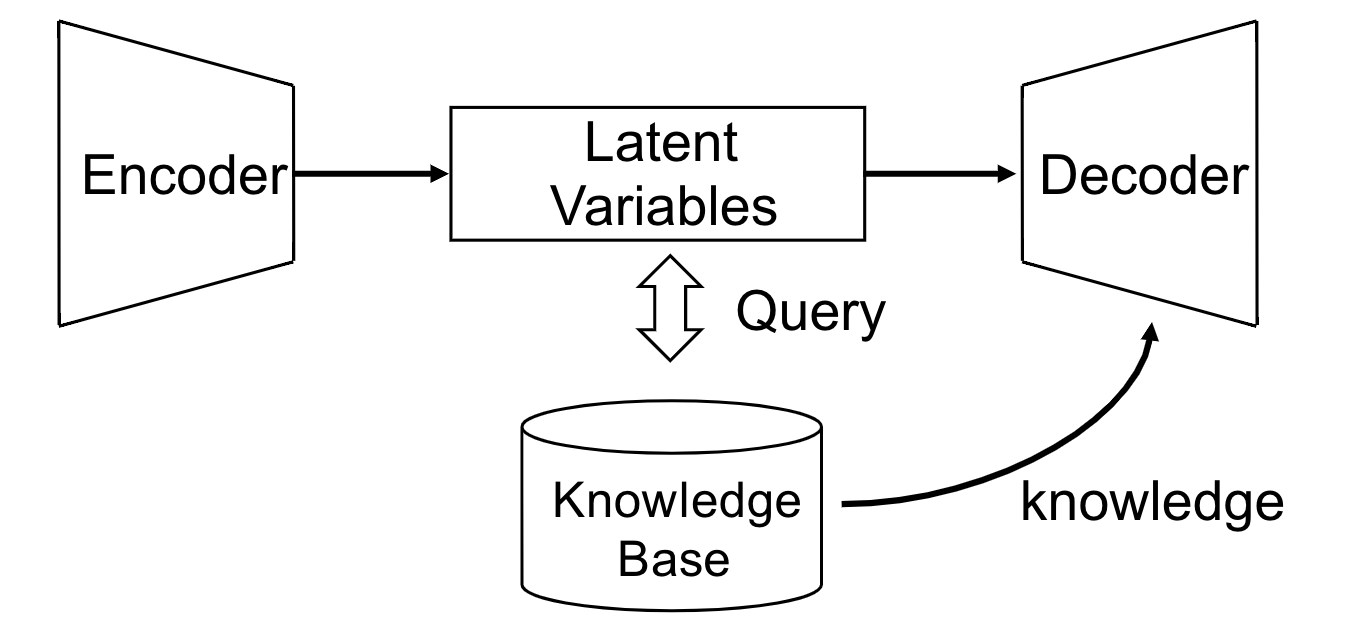
\includegraphics[scale = 0.35]{end2endframework.png}
    \caption{Framework of end-to-end dialog systems. It first encodes natural language context to obtain some latent variables, which can be used for KB query. Then based on the latent variables and query results, the decoder generates a natural language response}
    \label{end2endframework}
\end{figure}
\subsection{End-to-End Methods}
Generally speaking, the components in the pipeline system are individually optimized. This modular structure leads to complex model design, and the performance of each individual component does not necessarily translate into the progress of the entire system \cite{gao2018neural}. The end-to-end  approaches for task-oriented dialog systems are inspired by the researches on  open-domain  dialog  systems,  which use neural  models to build the system in an end-to-end manner without modular design, as shown in Figure \ref{end2endframework}. Most of these methods utilized sequence to sequence models as the infrastructural framework, which is end-to-end differentiable and can be optimized by gradient-based methods. In  most  existing  end-to-end  approaches,  the models are trained to maximize the prediction  probability of response in  the collected  data.   Wen  et  al.  \cite{DBLP:conf/eacl/Rojas-BarahonaG17}  proposed  a  modularized end-to-end model in which each component is modeled using neural networks, which makes the model end-to-end  differentiable Bordes  et  al. \cite{bordes2016learning}formalized  the  task-oriented dialog as a reading comprehension task by regarding the dialog history as context, user utterance as the question,and system response as the answer. In this work, they utilized end-to-end memory networks for multi-turn inference. Madotto et al. \cite{madotto2018mem2seq} took a similar approach and further feedthe knowledge base information into the memory networks.In \cite{eric2017key}  a  new  memory  network  structure  named  key-valuememory networks is introduced to extract relevant information from KB through key-value retrieval. Lei et al. \cite{lei2018sequicity} proposed a two-step seq2seq generation model which by passed the structured dialog act representation, and only retain the dialog state representation. In their method, the model first encodes the dialog history and then generates a dialog state using LSTM and CopyNet.  Given the state, the model then generates the final natural language response.

One major drawback of the above methods is that they often require large amounts of training data, which is expensive to obtain.  Furthermore, they cannot fully explore the state-action space since the model only observes examples in the data. Therefore, reinforcement learning methods are introduced to mitigate these issues \cite{lei2018sequicity,zhao2016towards,williams2017hybrid,dhingra2016towards,li2017end,liu2017iterative}.  In \cite{zhao2016towards}, there is an end-to-end  model  that  takes  the  natural  language  utterance as input and generates system dialog act as a response.   In this method, there is no explicit state representation. Instead,they used LSTM to encode the dialog history into a state vector and then use DQN to select an action. Williams et al. \cite{williams2017hybrid} proposed LSTM-based hybrid code networks (HCN), which supports self-defined software.
\section{Evaluation}

Evaluation of task-oriented dialogue systems is still an active research field because of the multiplicity of possible acceptable responses an agent could give. Most evaluation studies follow  the  PARADISE \cite{walker1997paradise}  framework. It estimates the user satisfaction from two aspects. One is dialog cost that measures the cost incurred in the dialog, such as the number of turns. The other one is task success that evaluates whether the system successfully solves the users problem.   The approaches to evaluate a task-oriented  dialog  system  can  be roughly grouped into the following three lines.
\subsection{Automatic Evaluation}
Automatic evaluation is widely advocated since it is quick, cheap, and objective. A bunch of well-defined automatic metrics have been designed for different components in the system. For language understanding, slot F1 and intent accuracy are used. For dialog state tracking, the evaluation metrics include slot accuracy and joint state accuracy in general.For policy optimization,inform rate,match rate and task success rate are used. For language generation, metrics such as BLEU and perplexity are applicable. Detailed definition of these metrics can be found in \cite{takanobu2020your}. All the models can be optimized against these metrics via supervised learning. However, each component is trained or evaluated separately in this way. Moreover, it assumes that the model would be fed with the ground truth from upstream modules or last dialog turn in the training process, but this assumption is invalid in real conversation.
\subsection{Simulated Evaluation}
In addition to training RL-based agents, a user simulator mimicking user behaviors in the task-oriented dialog also enables us to evaluate a trained dialog system. This is because,distinct from open-domain dialog systems, user goals in task-oriented dialog systems are somehow “enumerable” so that it is feasible to exhaustively leverage domain expertise to build a user simulator, which can provide human-like conversational interaction for simulated evaluation. The metrics used in the simulated evaluation includes task success rate, dialog length, average rewards, etc. Simulated evaluation has been widely applied in the recently proposed dialog system platforms, such as PyDial \cite{ultes2017pydial} and ConvLab \cite{lee2019convlab,zhu2020convlab}. The main advantage of simulated evaluation is that (1) the system can be evaluated in an end-to-end fashion; (2) multi-turn interaction is available during inference; (3) synthetic dialog data can be efficiently generated for evaluation at no cost. Similar to dialog policy optimization, the main challenge of employing simulated evaluation is to build a good user simulator that can mimic real user behaviors as much as possible. Meanwhile, how to evaluate the user simulator also remains an ongoing research direction\cite{pietquin2013survey}.
\subsection{Human Evaluation}
Simulated evaluation is efficient to evaluate the system performance with automatic, simulated interactions.Even though having a perfect user simulator, we still require human judgement for more complete evaluation on, e.g. covariate shift between the simulated environment and real conversation \cite{liu2018adversarial} and the quality of response generation \cite{wen2016network}, to assess real user satisfaction. Human evaluation metrics include task success rate, irrelevant turn rate, redundant turn rate, user satisfaction score, etc. The researchers generally hire human users on the crowd-sourcing platform, and human evaluation can be conducted in the following two ways. One is indirect evaluation that asking the annotators to read the simulated dialog between the dialog system and the user simulator, then rate the score \cite{shi2019build } or give their preference among different systems \cite{takanobu2019guided} according to each metric. The other one is direct evaluation that the participants are asked to interact with the system to complete a certain task, give their ratings on the interaction experience. For example, language understanding that evaluates whether the dialog agent understands user input, and response appropriateness that evaluates whether the dialog response is appropriate during the conversation, are assessed in the DSTC8 competition\cite{li2020results}.
\section{Challenges}
\subsection{Data Efficiency}

Different from the research in open-domain dialog systems, data-driven approaches for task-oriented dialog systems often require fine-grained annotations to learn the dialog model in a specific domain, e.g., dialog act and state labels. However, it is often difficult to obtain a large-scale annotated corpus in a specific domain since (1) collecting a domain-specific cor-pus is more difficult than in the open-domain setting due to its task-specific nature, and (2) annotating fine-grained labels requires a large amount of human resources which is very expensive and time-consuming. Therefore, we have to face the problem of improving the data efficiency of building task-oriented dialog systems, particularly in low-resource settings.

\subsubsection{Transfer Learning}

Transfer learning relaxes the assumption of traditional machine learning that the training data and testing data should be sampled independently from an identical probability distribution, thus it can be applied to discover domain-invariant intrinsic features and structures underlying two different but related domains, which establishes successful transfer and reutilization of supervised information across domains. 

The same problem often occurs in task-oriented dialogue systems. For example, in the case of limited data in the hotel field, how does the restaurant reservation dialogue system adapt to hotel reservations? In this case, the ontologies of the two domains are similar, sharing many dialogue behaviors and slots. In this case, transfer learning can greatly reduce the amount of target data required for this adaptation.

Cross-lingual transfer learning methods are recently proposed. In \cite{schuster2018cross}, Schuster et al. studied three different cross-lingual transfer methods: (1) translating the training data, (2) using cross-lingual pre-trained embeddings, and (3) a novel method of using a multilingual machine translation encoder as contextual word
representations. MLT \cite{liu2020attention} is a novel zero-shot adaptation method for cross-lingual task-oriented dialogue systems which leverages very few task-related parallel word pairs
to generate code-switching sentences for learning the interlingual semantics across languages/

For domain transfer, a novel\cite{mrkvsic2015multi}proposed to learn the dialog state tracking model through multi-task learning on multiple domain datasets to transfer knowledge across domains, which can improve the performance on all tasks. In \cite{ilievski2018goal}, Ilievski et al. proposed to directly transfer the parameters of shared slots from the source domain model to initialize the target model. Chen et al. \cite{chen2018policy}proposed to model dialog agent using several slot-dependent agents and a slot -independent agent to track the private and public slots across different domains. In \cite{rastogi2017scalable,ren2018towards}, the parameters of DST models are shared across domains and is independent of predefined value sets. Therefore, the model is able to transfer to previously unseen domains.
 \subsubsection{Unsupervised Methods}
 
A key problem in the learning of dialogue strategies is to estimate the reward signal, which is difficult to obtain in practical applications. Therefore, establishing a reward estimation model is necessary for dialogue strategy learning, especially during RL training. By treating the dialogue strategy as a generator and the reward function as a discriminator, a Generative Adversarial Network (GAN) can be used to learn the reward function in an unsupervised manner.  Liu et al.  \cite{liu2018adversarial} first used GAN to learn a binary reward function by discriminating simulated from real user dialogs.  Xu et al.  \cite{xu2019unsupervised} extended this idea for detecting dialog failure by using the predicted reward as an indicator of failure.  Su et al.  \cite{su2016line}used another way for reward estimation using Gaussian Process. By modeling the uncertainty of predicted reward,  the model can actively re-quire human intervention on potential failure cases.  In their experiment, the requirement for human intervention dramatically decreases with the reduction in the uncertainty of re-ward  estimation,  which  remarkably  relieve  manual  annotation.

Recently, pre-training methods show superior performance on many NLP tasks. In such approaches, extensive linguistic features  can  be  transferred  from  large-scale  unlabeled  copora using unsupervised pre-training tasks, such as mask language modeling (MLM) and next sentence prediction (NSP).Wolf et al. \cite{wolf2019transfertransfo} followed this way by first pre-training a trans-former model on large-scale dialog data and then fine-tuningthe model on a personalized dialog task with multi-task learn-ing.  Budzianowski et al.  \cite{budzianowski2019hello} further explored this idea to task-oriented dialog without explicit standalone dialogue pol-icy and generation modules. In this work, the belief state and database state are first converted to natural language text and then  taken  as  input  to  the  transformer  decoder  besides  the context
\subsection{Multi-turn Dynamics}
Compared with open-domain dialogue systems, a major feature of task-oriented dialogue systems is the emphasis on multi-turn state-action dynamics, which is mainly related to dialogue management (DST and strategy). In a task-oriented dialogue system, the completion of a specific task is critical. Therefore, the dialog management research responsible for tracking the dialogue status and dialogue process is the backbone of the dialogue system.
Recent studies on the dialog management of task-oriented dialog systems are mainly focused on the following topics: (1)generative DST with value decoder for free-form slots, (2) dialog planning for better sample efficiency in policy learning,and (3) user goal estimation for predicting task success and user satisfaction.

\subsubsection{Generative DST}
Dialog state tracker plays a central role in task-oriented dialog systems by tracking of a structured dialog state representation at each turn. Most recent DST studies applied a word-level structure by taking natural language as input with-out NLU, which may avoid the errors propagated from the NLU component. In early neural DST methods,belief state is widely adopted for dialog state representation \cite{henderson2014word}, which maintains a distribution over all possible values for each slot.Therefore, early methods commonly formulated DST as a classification task \cite{mrkvsic2016neural,mrkvsic2015multi,henderson2013deep,zhang2019memoryzhang2019neural}.

Zhong et al. \cite{zhang2019neural} proposed to share parameters across slots and learn slot-specific features through a globally-locally self-attention mechanism, which can generalize to rare values with few training data. However, the rare values are still in-vocabulary words. Lei et al.\cite{lei2018sequicity} use a seq2seq model with two-stage CopyNet to generate belief spans and response at the same time, which obtain satisfactory results in OOV cases. In the first stage, a belief state CopyNet\cite{gu2016incorporating} takes the user utterance as input and generates a be-lief state span. Then in the second stage, based on the utterance and belief span, another CopyNet generates the response utterance.

Recently, some multi-domain datasets are proposed to promote the research in this direction \cite{budzianowski2018multiwoz,rastogi2020towards}. Compared to single-domain tasks, the DST in multi-domain scenario has to predict the domain of slot values. Wu et al . proposed TRADE\cite{rastogi2020towards}, a transferable multi-domain DST using seq2seq model with CopyNet \cite{gu2016incorporating} to predict values. The parameters are shared across domains, enabling zero-shot DST for unseen domains. COMER \cite{ren2020scalable} further reduces the computation complexity of value decoding by first deciding the domain and slot, and then decoding the value. In the decoding of the above methods, they first input the domain and slot names to the decoder, and then decode the value. If we take the domain and slot names as a form of “question”, then the model can be regarded as a question answering model by taking the previous turns as context, domain-slot names as question and the value as answer.

\subsubsection{Dialog Planning}
Model-free RL methods dominated the early studies of neural dialog policy by learning through interaction with real users\cite{mnih2015human,williams2017hybrid,dhingra2016towards}. It is data-hungry, requiring a large amount of interactions to train a policy model effectively. One common solution is to use user simulators \cite{schatzmann2007agenda,li2016user}. However, the user simulator is not able to fully mimic real human conversation behaviors, and its inductive bias may lead to sub-optimal models that perform poorly in real human conversation \cite{shi2019build} .

In order to alleviate these problems, model-based RL methods are proposed to model the environment so as to plan the dialogue strategy learning. In the model-based RL method, the environment is modeled to simulate the dynamics of the dialogue. Then in the RL training phase, the dialogue strategy is alternately trained by learning from real users and planning using the environment model. Peng et al.\cite{peng2018deep} proposed the Deep Dyna-Q (DDQ) framework, which first integrated model-based planning for task-oriented dialogue systems.

The above methods for planning are referred to as background planning, which improves the policy through training on simulated experience with the world model. Another line of planning-based research is decision time planning, which directly decides which action to take in a specific state St based on some simulated experience. The simulated future steps can provide extra hints to facilitate decision making. Planning used in this way can look much deeper than one-step ahead at decision time, which is common in human activities. Taking the chess game for example, the players often conduct mental simulation by looking several steps ahead and then decide how to move the pieces. Some works \cite{lewis2017deal,yarats2018hierarchical} introduce dialog roll out planning into negotiation dialogs, in which the agent simulates complete dialogues in a specific state St for several candidate responses to get their expected reward, and the response with the highest reward will be taken. Instead of completing the dialogs and obtaining explicit rewards, Jiang et al. \cite{jiang2019towards} proposed to look only several limited steps ahead and use those steps as additional features for the policy model to alleviate decision making.

\subsubsection{User Goal Estimation}
In RL-based dialog models, the user's goal is crucial for policy learning. Reward signal is an indirect reflect of the user's goal since it gives the user's satisfaction of a dialog. One typical approach of reward function definition is to assign a large positive reward at the end of a successful session and a small negative penalty for each turn to encourage short conversations \cite{su2018reward}. However, in real-world applications where user goals are not available, such rewards cannot be effectively estimated. Another problem is that the reward signal is inconsistent when calculated objectively through predefined rules or subjectively judged by real users. In order to alleviate the above problems, there are some studies to learn independent reward functions to provide reliable supervision signals.

One method for reward estimation is off-line learning with annotated data \cite{yang2012predicting}. By taking the dialog utterances and intermediate annotations as input features, reward learning can be formulated as a supervised regression or classification task. The annotated reward can be obtained from either human annotation or user simulator. However, since the input feature space is complicated, a large amount of manual annotation is required, which is too costly.

To resolve the above problems, there is another line of work using on-line learning for reward estimation \cite{su2016line}. Reward estimation is often formulated as a Gaussian Process regression task, which can additionally provide an uncertainty measure of its estimation. In this setting, active learning is adopted to reduce the demand for estimating real reward signals in which the users are only asked to provide feedback when the uncertainty score exceeds a threshold. In other cases, when the estimation uncertainty is small, the estimated reward is utilized.
\subsection{Ontology Integration}
One of the main problems of task-oriented dialogue systems is to integrate dialogue ontology into dialogue models, including domain schema and knowledge bases. In most previous methods, domain schema are pre-defined and highly dependent on the corpus they use. For example, the slot of the restaurant domain contains address area, dish type, price range, etc. Querying the database and retrieving the results is essential for task-oriented dialogue systems to make decisions and produce appropriate responses. Recently, there have been many efforts to integrate external databases or API calls.

However, due to the large-scale task domain, the ontology integration of task-oriented dialogue models becomes more challenging. Although pre-defined ontology can be considered in model design, these methods are coupled with domain schema and cannot be easily transferred to new tasks. Although it is proposed to add an end-to-end model to alleviate the pattern integration problem, it is not easy to involve contextual information and knowledge base, because unlike the pipeline method, there is no explicit dialog state representation to generate explicit knowledge basic queries.
\subsubsection{Schema Integration}

Integrating the schema into a dialog model is critical for task-oriented dialog, since the value prediction of NLU and DST, and  the action selection in Policy are highly  dependent  on the domain schema.  Early methods for NLU use classification for intent detection and sequence labeling for slot-value recognition. Therefore, the schema integration are mainly reflected in the model output layer design, e.g., one class for each intent. Early DST methods utilized a similar way by giving a value  probability distribution on the value  vocabulary for each slot (also  known  as  belief  state). For NLG methods, the inputs are often structured dialog acts, and the encoder input structure is highly dependent on the representation structure.

The above schema integration methods basically couple the schema and model design together,  yield poor scalability  and  domain  generalization. Recently, there are  many methods trying to untie the domain scheme and model design. Convlab  \cite{lee2019convlab}  provides  additional  user  dialog  act  annotation in the MultiWOZ \cite{budzianowski2018multiwoz}dataset to enable developers to apply NLU models in multi-domain, multi-intent settings. While most DST makes assumption that a slot in a belief state can only be mapped to a single value within a single turn, COMER \cite{ren2020scalable}extends the representation of dialog states with priority operator that considers the user’s preference on slot values. For NLG  task,  Peng  et  al.   \cite{peng2020few} proposed  SC-GPT,  which treats the structured dialog act as a sequence of tokens, and feeds the sequence to the generation model.  By pre-training on large-scale da-response pairs, the model is able to capture the semantic structure of the sequence-based dialog act representation.
\subsubsection{Knowledge Base Integration}

For task-oriented dialogue systems, it is very important to query external knowledge bases to obtain the information that users query. Early models or pipeline systems retrieve items from the knowledge base by issuing queries based on the current dialog state during dialog interaction, which requires some manual effort. Due to the increasing task complexity in task-oriented scenarios, training end-to-end dialogue systems without intermediate supervision will be more attractive. However, unlike the pipeline method, there is no clear structured dialog state representation in the end-to-end method. Therefore, the knowledge base interaction is carried out by using the intermediate latent representation of the model, and is seamlessly trained through end-to-end training.

CopyNet and end-to-end memory networks are widely used for integrating knowledge into dialog systems through the attention mechanism. The copy mechanism, however, can also be regarded as a memory network in which the encoder hidden states consist of the memory units. Eric et al. \cite{eric2017copy}presented a copy-based method depending on the latent neural embedding to attend to dialog history and copy relevant prior context for decoding. However, they can only generate entities that are mentioned in the context. More recent works use memory networks for prior dialog context and knowledge integration \cite{madotto2018mem2seq,wu2019global}. In such approaches, the dialog con-text and knowledge base are modeled into two memory nets.Then in the decoding phase, the decoder's hidden state is used to selectively query and copy information from those memory nets. A key problem in such a method is that dialog con-text and knowledge base are heterogeneous information from different sources. Lin et al. \cite{lin2019task} proposed to model heterogeneous information using historical information, which is stored in a context-aware memory, and the knowledge base tuples are stored in a context-free memory. In \cite{qin2019entity }, a two-step KB retrieval is proposed to improve the entities' consistency by first deciding the entity row and then selecting the most relevant KB column.

\section{Conclusion and Future Trends}
In this paper,  we review the recent advancements on task-oriented dialog systems and discuss three critical topics: data efficiency, multi-turn dynamics, and knowledge integration. Despite these themes, there are still some interesting and challenging questions. We finally conclude some future trends in task-oriented dialogue systems:

\textbf{Pre-training Methods for Dialog Systems.}
Data scarcity is a key challenge in building a task-oriented dialogue system. On the one hand, collecting enough data for a specific area is time-consuming and expensive. On the other hand, the task-oriented dialogue system is a composite NLP task. It not only learns grammar, reasoning, decision-making and language generation from offline data, but also learns from online interaction with users, presenting more fine-grained requirements. Data annotation and model design.

Recently, pre-trained models have shown excellent performance in many NLP tasks \cite{devlin2018bert,DBLP:conf/naacl/PetersNIGCLZ18,radford2018improving}. In this case, the basic model is first pre-trained on a large-scale corpus through some unsupervised pre-training tasks, such as mask language model and next sentence prediction. In the pre-training stage, the basic model can capture implicit language knowledge and learn from a large-scale corpus. Using this implicit knowledge, the basic model can quickly adapt to the target task by simply fine-tuning the target task's data. This idea can also be applied to task-oriented dialogue systems to transfer general natural language knowledge corpus to specific dialogue tasks on a large scale. Some early studies have shown the possibility of using pre-trained models to model task-oriented dialogue\cite{peng2020few,wolf2019transfertransfo,budzianowski2019hello,mehri2019pretraining}.

\textbf{Domain Adaptation}
Unlike open domain dialogue, task-oriented dialogue is based on a well-defined domain ontology, which constrains agent actions, slot values and knowledge bases for specific tasks. Therefore, in order to complete a task, the model of the dialogue system is highly dependent on the domain ontology. However, in most existing studies, this ontology knowledge is hard-coded into the model. For example, dialogue behavior types, slot value vocabulary and even slot-based belief states are all embedded in the model. This hard-coded ontology embedding raises two problems: (1) Human experts are required to analyze tasks and integrate domain ontology into model design, which is a time-consuming process. (2) The existing model cannot be easily transferred to another task. Therefore, decoupling domain ontology and dialogue model to obtain better adaptive performance is a key issue. One ultimate goal is to achieve zero-shot domain adaptation, which can directly construct a dialogue system with a given ontology just like a human, without any training data.

\textbf{Robustness}.The robustness of deep neural models has always been a challenging problem because existing neural models are susceptible to simple input disturbances. For task-oriented dialogue systems, robustness is also a key issue, which mainly comes from two aspects: (1) On the one hand, task-oriented dialogue highly relies on domain ontology. Therefore, in many studies, training data is limited to reasonable examples with little noise. However, models that are strained in this particular way often fail to meet the requirements in practical applications. In these applications, there are many out-of-domain or out-of-distribution inputs\cite{zheng2020out}, such as previously invisible slot values. A powerful dialogue system should be able to handle noise and previously invisible input after deployment. (2) On the other hand, the decision-making of the neural dialogue strategy model is uncontrollable. It is trained through offline imitation learning and online reinforcement learning. Robustness of decision-making is very important to its performance, especially for some special applications with low tolerance for errors, such as in the medical and military fields. Therefore, improving the robustness of neural dialogue models is an important issue. One possible approach is to combine robust rule-based methods with neural models, such as neural symbolic machines\cite{liang2016neural,segler2017neural}, which may make the model not only more robust, but also easier to interpret.

\textbf{End-to-end Modeling}
Compared with the pipeline method, end-to-end dialog system modeling has attracted more and more attention in recent years. It is easier to train end-to-end models without the need to explicitly model conversation states and strategies. However, existing end-to-end methods still require some intermediate supervision to improve model performance.

For example, in \cite{wen2016network}, a modular-based end-to-end frame-work  is  proposed  by  combining  pre-trained  components together and then fine-tuning all the components using RL in an end-to-end fashion, which still requires intermediate supervision such as dialog act and belief state at the pre-training phase. In \cite{lei2018sequicity}, although a seq-to-seq framework is proposed to avoid component barriers,  intermediate  output  named belief  spansis  still retained for explicit belief state modeling.  Therefore,the problem of modeling task-oriented dialog in a fully end-to-end  fashion,  without  intermediate  supervision and can seamlessly interact with the knowledge base,is still an open problem.

\clearpage
%%%%%%%%% REFERENCES
{\small
\bibliographystyle{ieee_fullname}
\bibliography{egbib}
}

\end{document}
